% !TeX root = ../dokumentation.tex
\setpagestylefoot
\renewcommand{\thefigure}{A\arabic{figure}}
\renewcommand\thelstlisting{A\arabic{lstlisting}}
\renewcommand\thetable{A\arabic{table}}

\appendix
\renewcommand{\thesection}{\Alph{section}}
\renewcommand{\thesubsection}{\Alph{section}.\Alph{subsection}}


% Quellenverzeichnis nach Literatur und Weblinks trennen
%\printbibliography[heading=subbibintoc,title={Literatur},nottype=online]
%\printbibliography[heading=subbibintoc,title={Weblinks},type=online]

% Quellenverzeichnis nicht trennen
\ifliteratur
    \printbibliography[heading=bibintoc,title={Quellen}]
\fi

% Nummer des Inhaltes mit \setcounter{figure}{"`Number"'} (figure, lstlisting or table) ändern wenn nötig

\addchap{\langanhang}
%Place for extra content

\section{Guidelines}
\subsection{Contribution Guideline} \label{contrib}
\begin{figure}[H]
    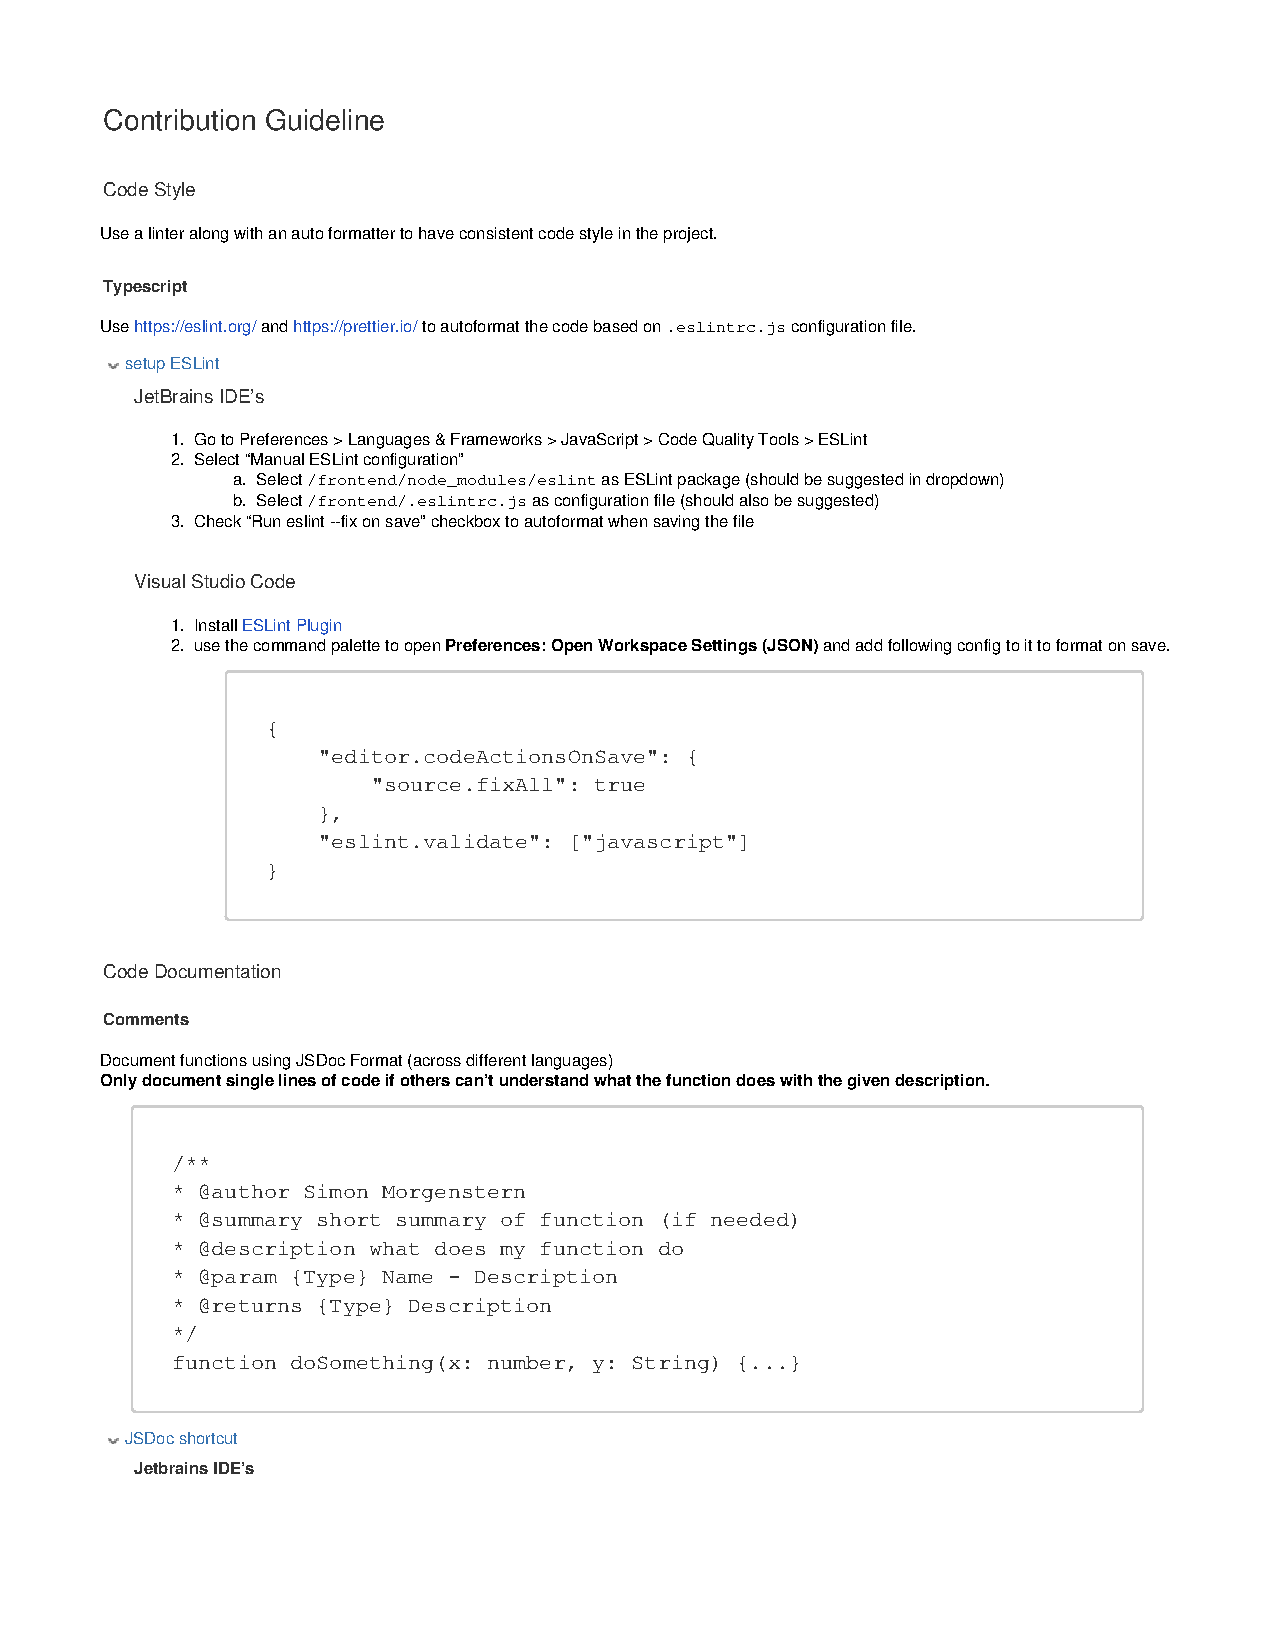
\includegraphics[width=\linewidth, page=1]{SKIOSA-ContributionGuideline.pdf}
    \caption*{Contribution Guideline - Seite 1}
\end{figure}
\begin{figure}[H]
    \includegraphics[width=\linewidth, page=2]{SKIOSA-ContributionGuideline.pdf}
    \caption*{figure}{Contribution Guideline - Seite 2}
\end{figure}

\subsection{Testing Guideline}
\begin{figure}[H]
    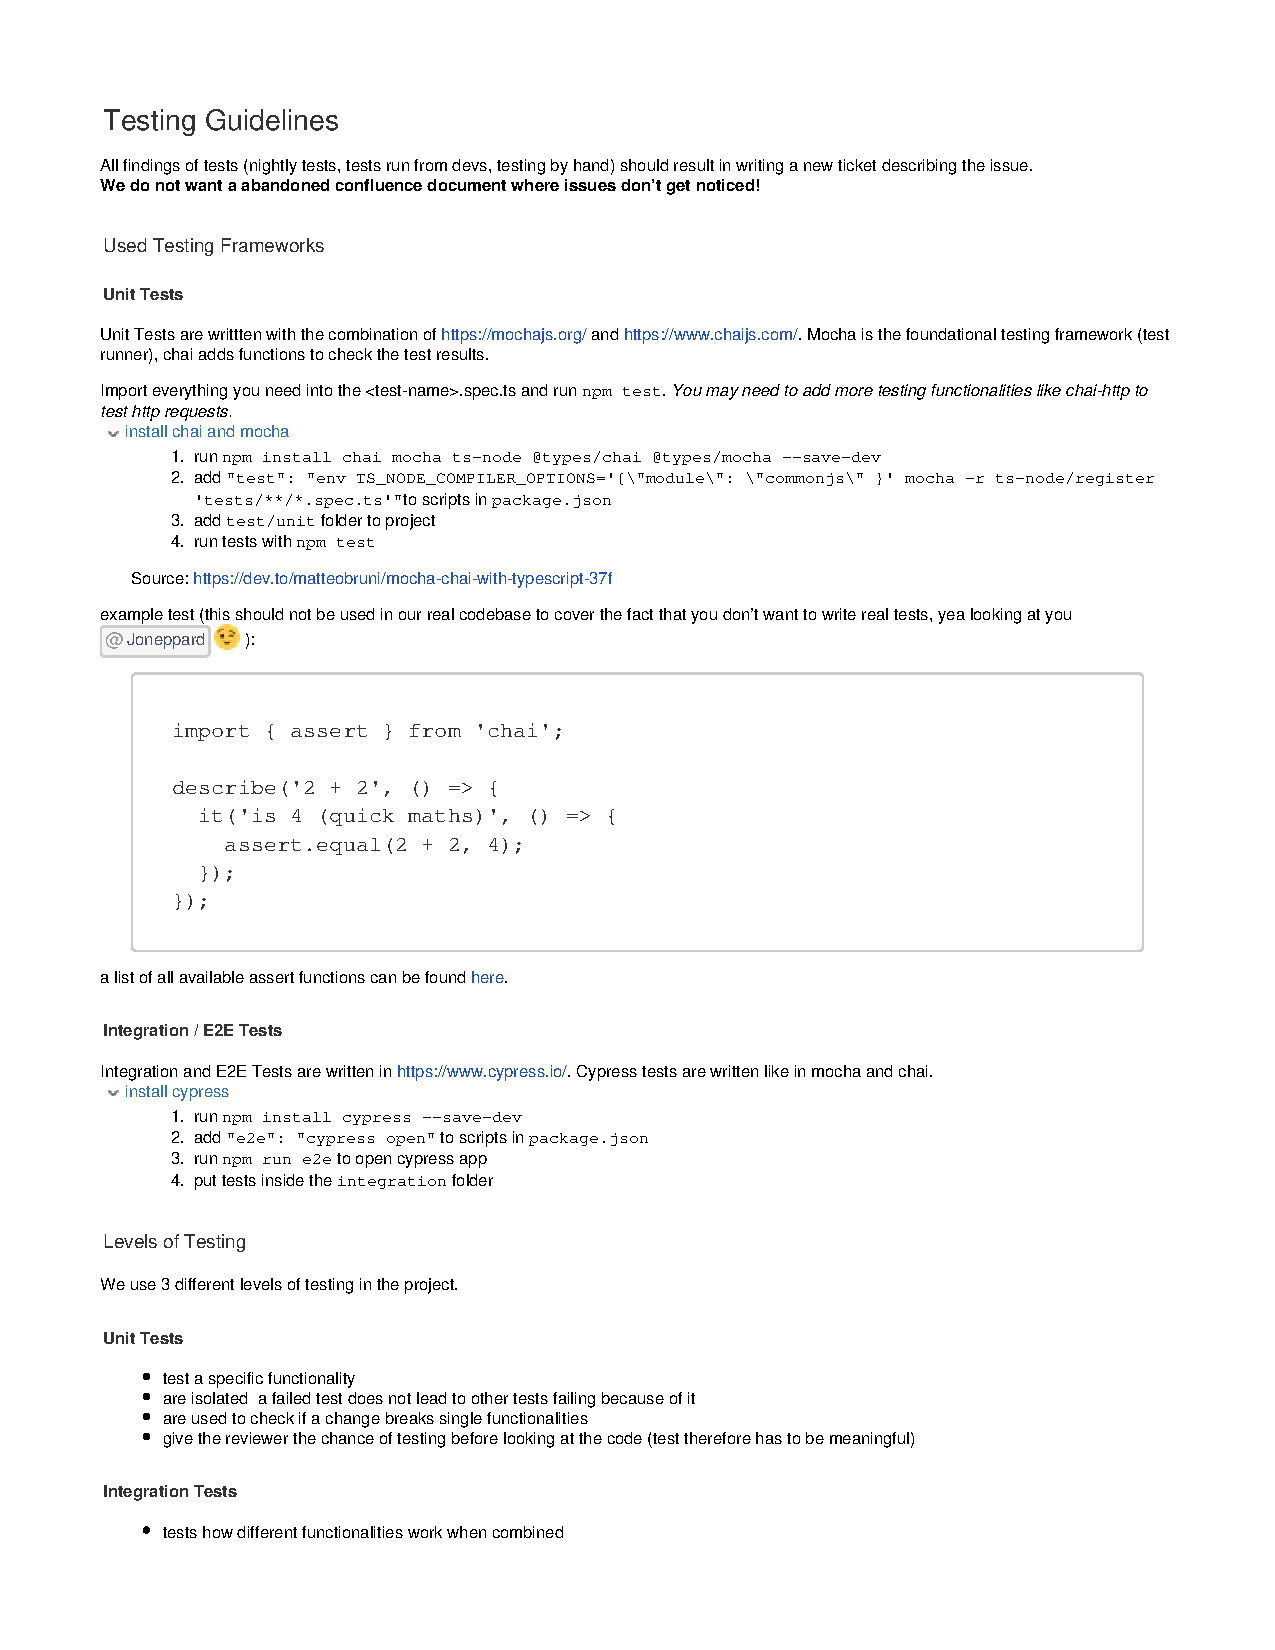
\includegraphics[width=\linewidth, page=1]{SKIOSA-TestingGuidelines.pdf}
    \caption*{Testing Guideline - Seite 1}
\end{figure}
\begin{figure}[H]
    \includegraphics[width=\linewidth, page=2]{SKIOSA-TestingGuidelines.pdf}
    \caption*{Testing Guideline - Seite 2}
\end{figure}

\section{Dokumentation der Software}
\subsection{Frontend}
\begin{figure}[H]
    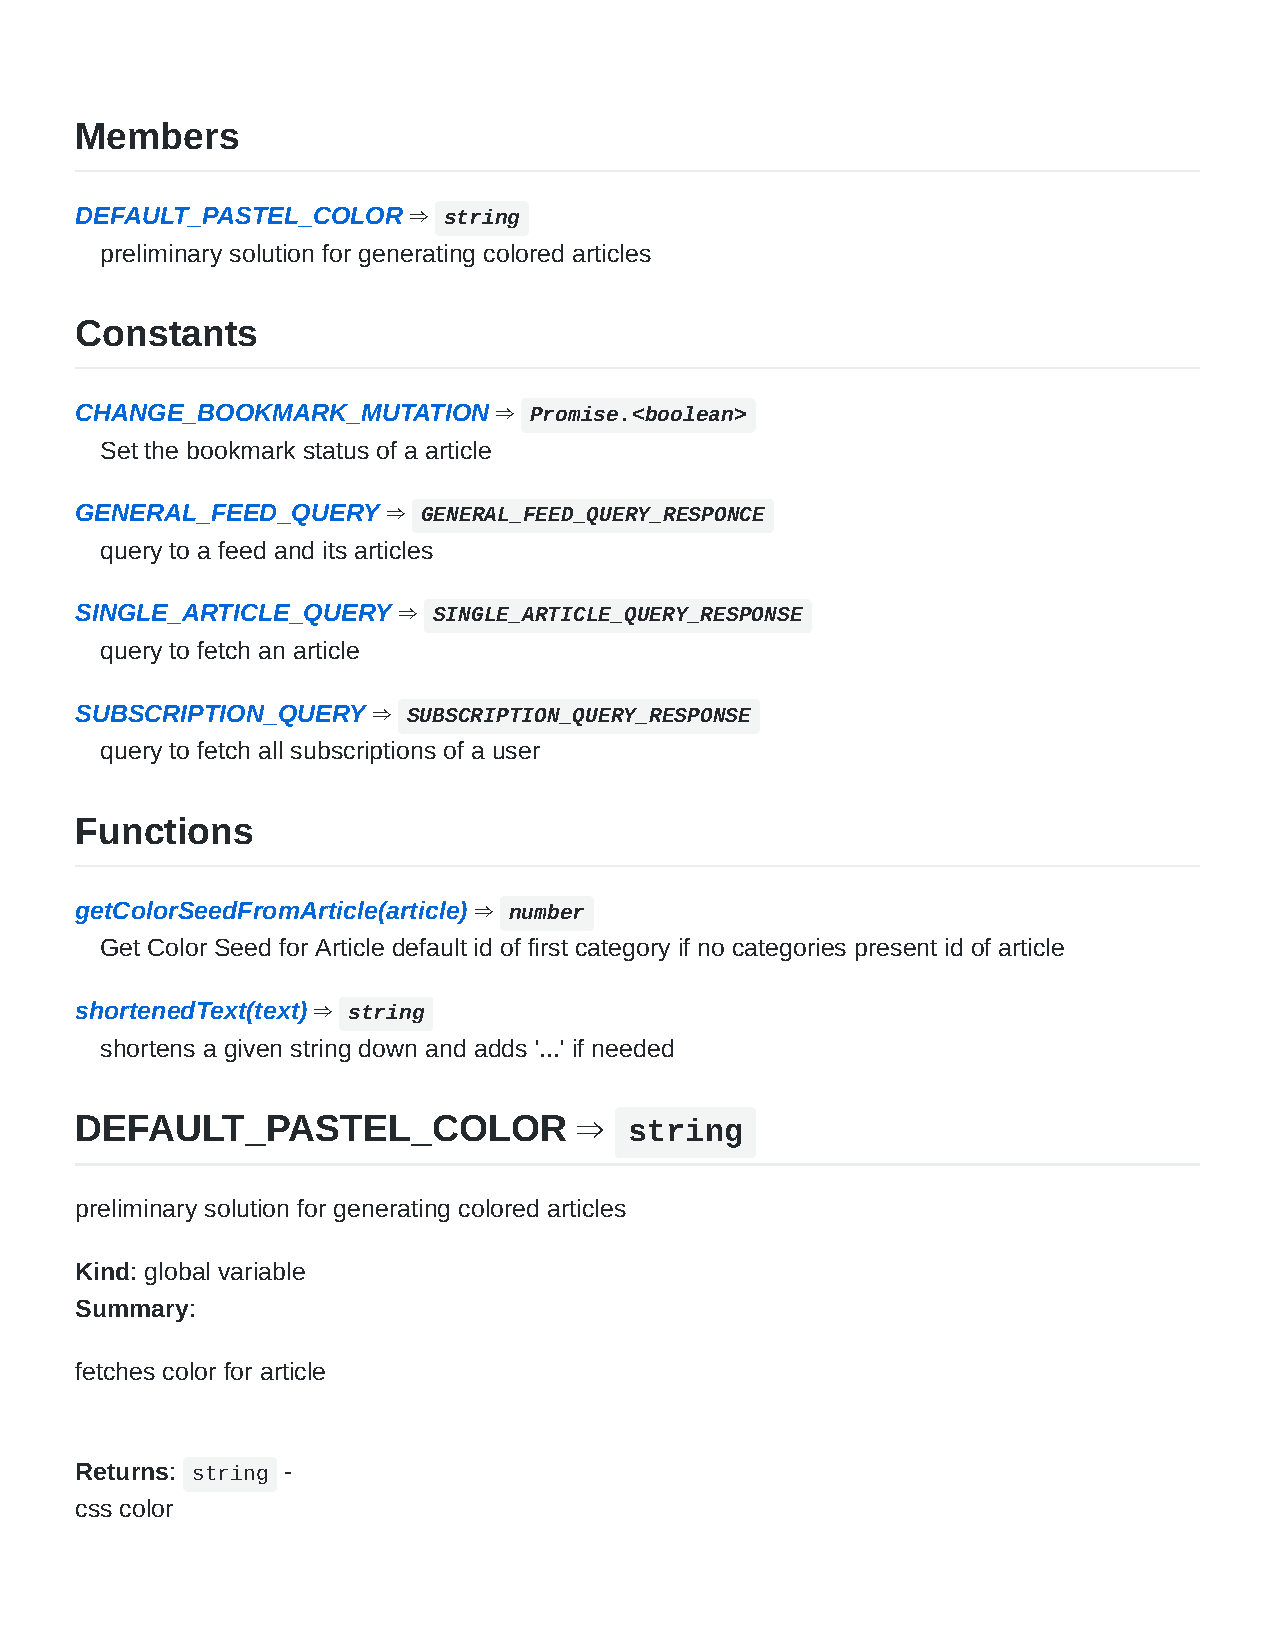
\includegraphics[width=\linewidth, page=1]{frontend.pdf}
    \caption*{Ausschnitt des Frontend JSDoc - Seite 1}
\end{figure}
\begin{figure}[H]
    \includegraphics[width=\linewidth, page=2]{frontend.pdf}
    \caption*{Ausschnitt des Frontend JSDoc - Seite 2}
\end{figure}
\begin{figure}[H]
    \includegraphics[width=\linewidth, page=3]{frontend.pdf}
    \caption*{Ausschnitt des Frontend JSDoc - Seite 3}
\end{figure}
\begin{figure}[H]
    \includegraphics[width=\linewidth, page=4]{frontend.pdf}
    \caption*{Ausschnitt des Frontend JSDoc - Seite 4}
\end{figure}
\begin{figure}[H]
    \includegraphics[width=\linewidth, page=5]{frontend.pdf}
    \caption*{Ausschnitt des Frontend JSDoc - Seite 5}
\end{figure}

\subsection{Core-Service}
\begin{figure}[H]
    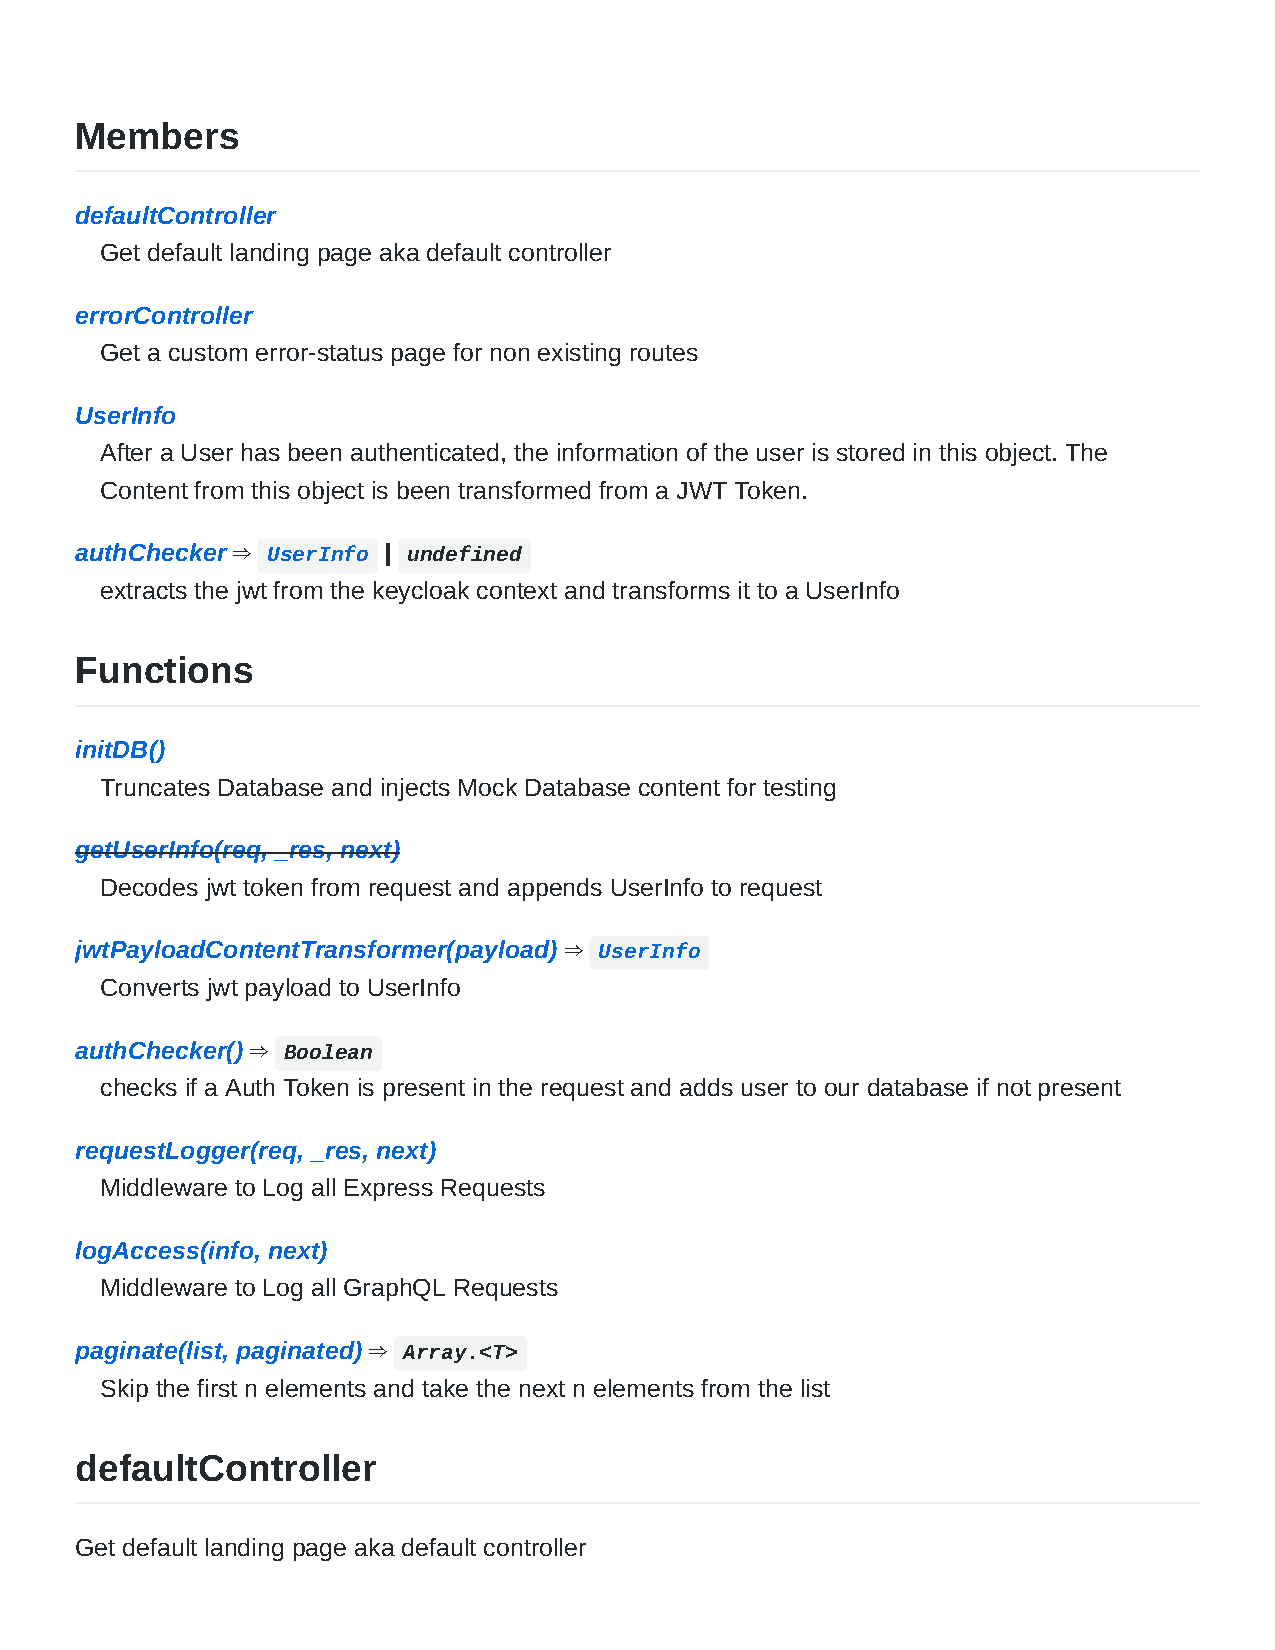
\includegraphics[width=\linewidth, page=1]{core_service_docs.pdf}
    \caption*{Ausschnitt des Core Service JSDoc - Seite 1}
\end{figure}
\begin{figure}[H]
    \includegraphics[width=\linewidth, page=2]{core_service_docs.pdf}
    \caption*{Ausschnitt des Core Service JSDoc - Seite 2}
\end{figure}
\begin{figure}[H]
    \includegraphics[width=\linewidth, page=3]{core_service_docs.pdf}
    \caption*{Ausschnitt des Core Service JSDoc - Seite 3}
\end{figure}
\begin{figure}[H]
    \includegraphics[width=\linewidth, page=4]{core_service_docs.pdf}
    \caption*{Ausschnitt des Core Service JSDoc - Seite 4}
\end{figure}
\begin{figure}[H]
    \includegraphics[width=\linewidth, page=5]{core_service_docs.pdf}
    \caption*{Ausschnitt des Core Service JSDoc - Seite 5}
\end{figure}
\begin{figure}[H]
    \includegraphics[width=\linewidth, page=6]{core_service_docs.pdf}
    \caption*{Ausschnitt des Core Service JSDoc - Seite 6}
\end{figure}

\subsection{Polling-Service}
\begin{figure}[H]
    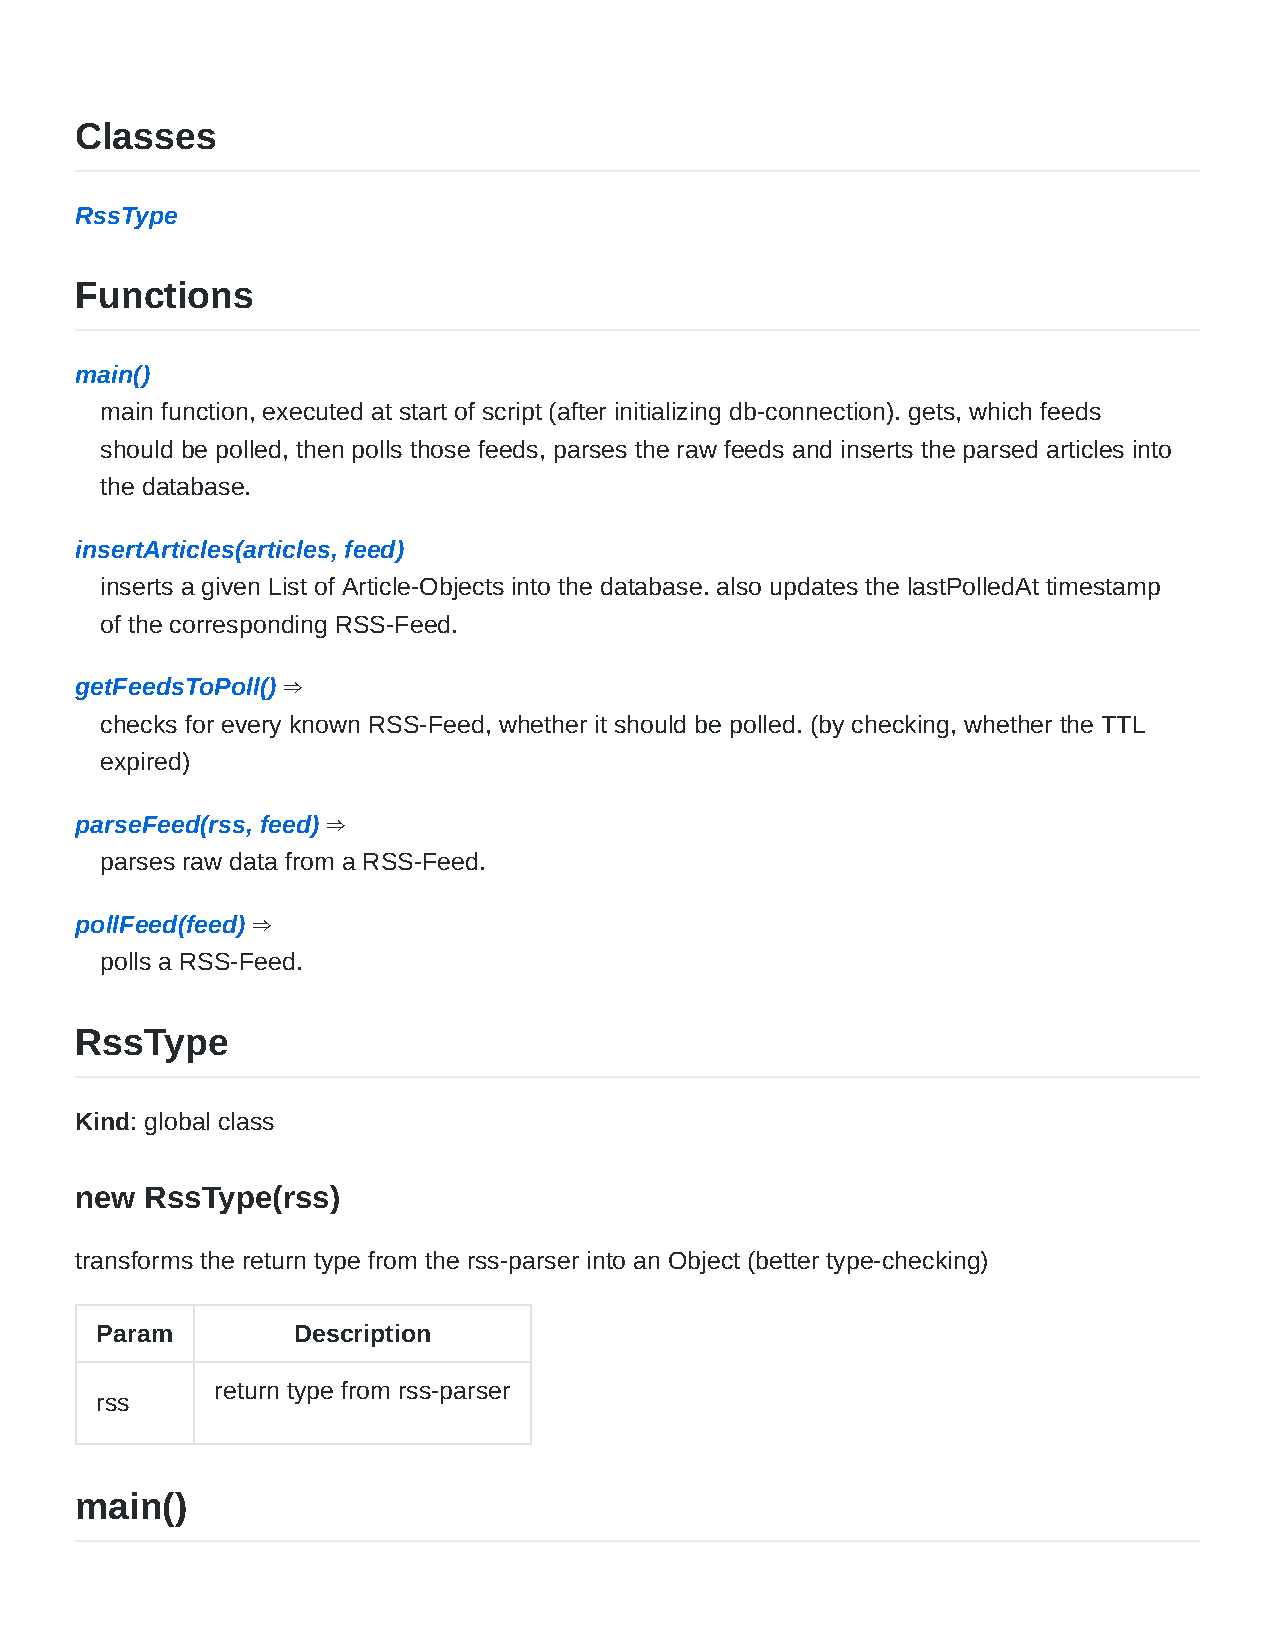
\includegraphics[width=\linewidth, page=1]{polling_service.pdf}
    \caption*{Ausschnitt des Polling Service JSDoc - Seite 1}
\end{figure}
\begin{figure}[H]
    \includegraphics[width=\linewidth, page=2]{polling_service.pdf}
    \caption*{Ausschnitt des Polling Service JSDoc - Seite 2}
\end{figure}
\begin{figure}[H]
    \includegraphics[width=\linewidth, page=3]{polling_service.pdf}
    \caption*{Ausschnitt des Polling Service JSDoc - Seite 3}
\end{figure}